It is a universal truth that visuals better appeal to the human mind than a group of numbers listed out. With visuals, it is easier for us to discern patterns and identify any flaws in the logic behind our mathematical calculations and equations. To visualize the different Discrete Distribution and True Measure Objects, the \href{https://qmcpy.org/}{QMCPy} Plot Projections function has been developed. This blog presents the different applications of this function.

\subsection*{What does the Plot Projections Function Do?}
A Discrete Distribution or True Measure object with $d \geq 2$ dimensions has a maximum of $d\times(d -1)$ 
dimensional pairings (for e.g: [2,3] and [3,2] are being considered separate parings). The Plot Projections function (referred to as plot\textunderscore proj) plots all or a subset of all the possible dimension pairings based on user argument. This function either takes a Discrete Distribution or True Measure Object at a time. It can also display extensibility by passing in a list of successfully larger samples (for e.g: [$2^{6}$,$2^{7}$,$2^{8}$]). 
 To display extensibility, plot\textunderscore proj function uses \href{https://matplotlib.org/stable/gallery/color/color_cycle_default.html}{the default prop\textunderscore cycle}, which is obtained from the rc parameters of Matplotlib. This default prop\textunderscore cycle contains a list of colors through which the plot\textunderscore proj function iterates over and displays extensibility. The list of colors is : blue, orange, green, red, purple, brown, pink, grey, yellow, cyan. The colors are stored in this order but in a hexadecimal format.
 \\\\ The parameters and plot examples of this function can be seen in the \href{https://github.com/QMCSoftware/QMCSoftware/blob/master/demos/plot_proj_function.ipynb}{Plot Projections Notebook}.
\subsection*{Setting up the QMCPy environment before utilizing the Plot Projections Function:}
 \lstinputlisting[style = Python]{PlotProjectionsFunction/code/initialization.py}
 \subsection*{The Different Applications of the Plot Projection Function:}
 \begin{enumerate}
     \item Here we show a two dimensional projection of an IID Object:
     \lstinputlisting[style = Python]{PlotProjectionsFunction/code/iid.py}
     \begin{figure}[H]
    \centering
    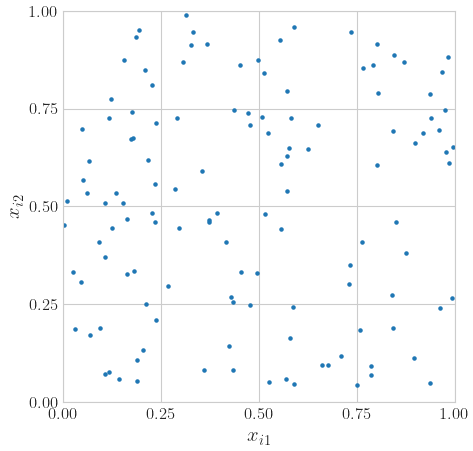
\includegraphics[width=0.55\linewidth]{PlotProjectionsFunction/Figures/iid.png}
    \end{figure}
    \item Here we show a two dimensional projection of a Gaussian Object and how the axes returned by the plot\textunderscore proj function can be manipulated by adding a horizontal and vertical line to denote the x and y axis respectively:
    \lstinputlisting[style = Python]{PlotProjectionsFunction/code/iid_gaussian.py}
     \begin{figure}[H]
    \centering
    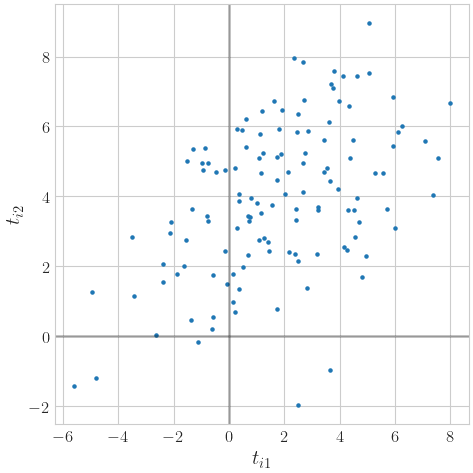
\includegraphics[width=0.55\linewidth]{PlotProjectionsFunction/Figures/iid_gaussian.png}
    \end{figure}
     \item Here we show certain specified dimensional projections (dimensions 1 and 2 on the x axes, dimensions 3 and 4 on the y axes) of a  Uniform Object with successively increasing numbers of points.  The initial points are in blue. The next additional points are in orange. The final additional points are in green:
    \lstinputlisting[style = Python]{PlotProjectionsFunction/code/halton_uniform.py}
     \begin{figure}[H]
    \centering
    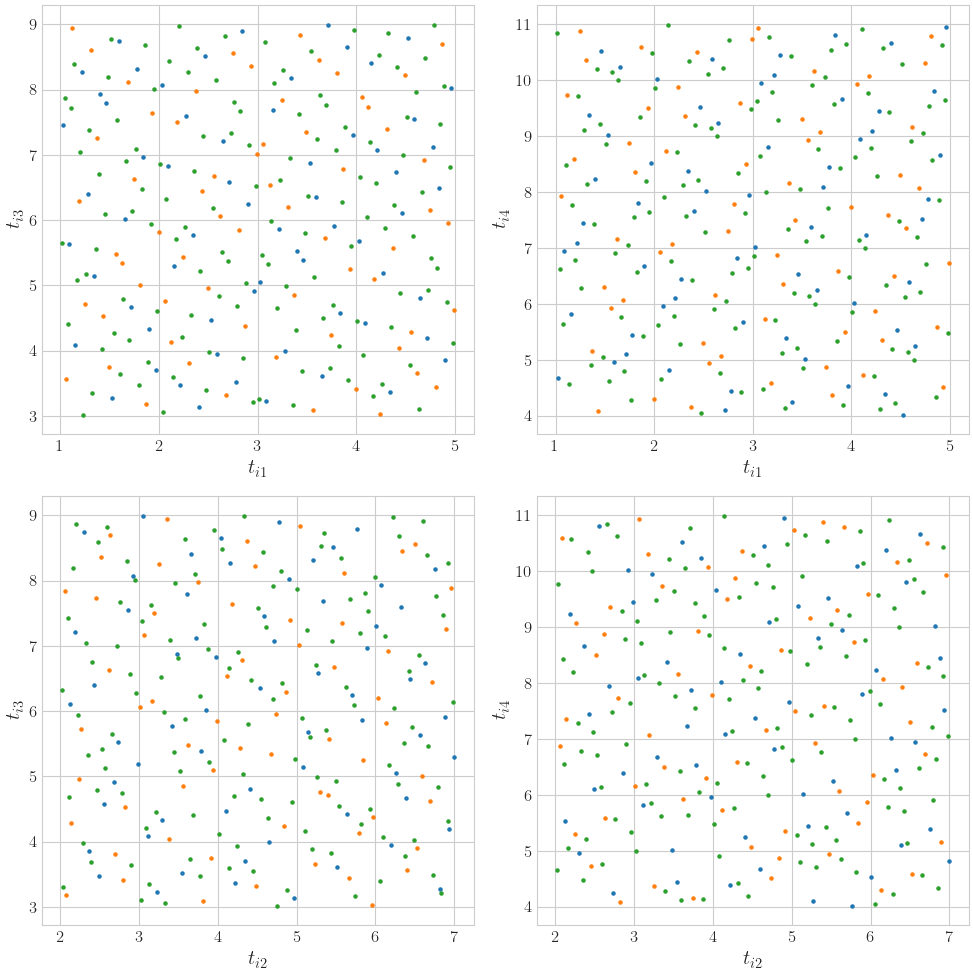
\includegraphics[width=0.9\linewidth]{PlotProjectionsFunction/Figures/halton_uniform.png}
    \end{figure}
    \item Here we show a four dimensional projection of a Halton Object  with successively increasing numbers of points.  The initial points are in blue. The next additional points are in orange. The final additional points are in green:
    \lstinputlisting[style = Python]{PlotProjectionsFunction/code/halton.py}
     \begin{figure}[H]
    \centering
    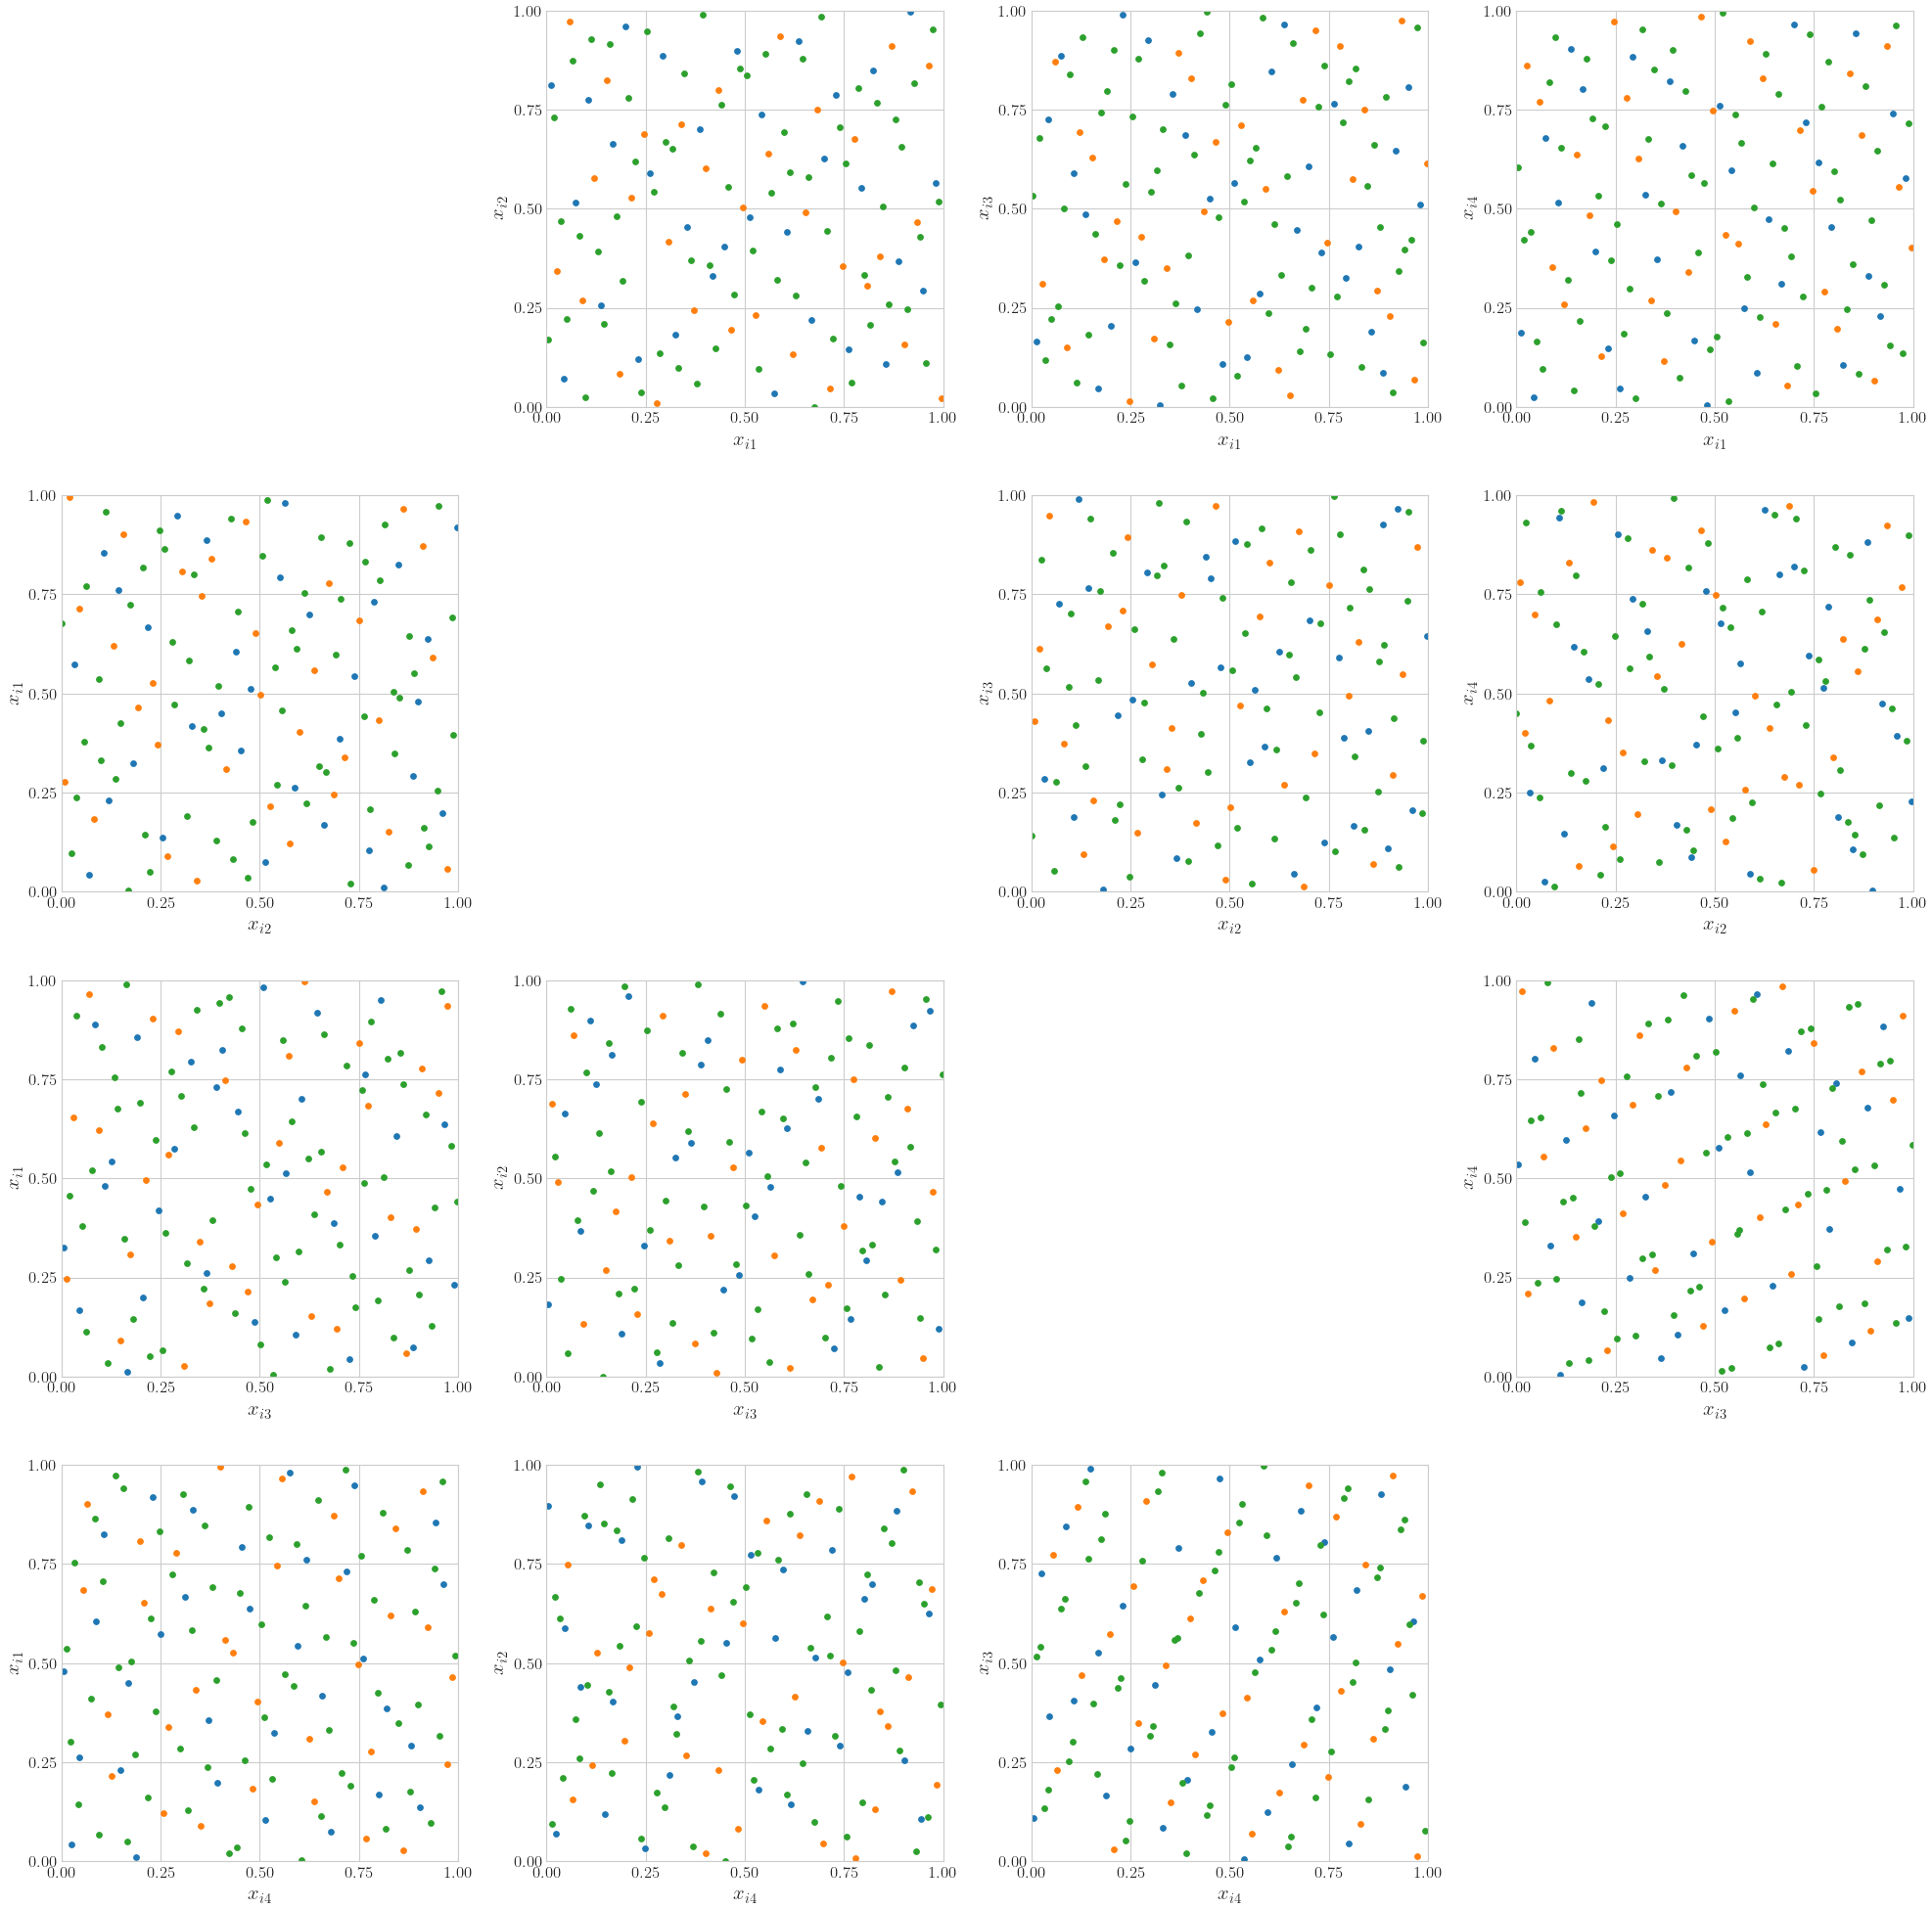
\includegraphics[width = 0.99 \linewidth]{PlotProjectionsFunction/Figures/halton.png}
    \end{figure}
 \end{enumerate}
 \subsection*{How this function benefits us:}
 In addition to making it easy to see the difference between different Discrete Distribution and True Measure Objects, this function consists of many features that makes it user-friendly and help generate a strong and precise visualization of the different Discrete Distribution and True Measure Object. For instance, the extensibility feature enables us to see how the space of the plot fills up, the marker\textunderscore size parameter helps make the samples/points bigger when plotting high-dimensional projections, and the math\textunderscore ind parameter allows the user to either input mathematical or python dimensions for the sampler based on one's preference.  This function could also be developed in the future to support other distributions such as Brownian Motion.
